\chapter{Evolution of Large Language Models}

\section{Historical Background of Language Models}

At the heart of Natural Language Processing (NLP) lie language models, whose primary function is to predict or estimate the probability of linguistic elements—such as words, phrases, or entire sentences—based on surrounding context. The development of language models has progressed through distinct stages. It began with rule-based models, which relied on hand-crafted linguistic rules to process language. This was followed by statistical language models (SLMs), which applied probability theory to model word sequences. Subsequently, neural language models (NLMs) emerged, utilizing neural networks to capture more complex language patterns and semantic relationships. Building on NLMs, pretrained language models (PLMs) were introduced, leveraging vast text corpora and self-supervised objectives to acquire broad linguistic knowledge. The latest stage in this evolution features large language models (LLMs)—a class of PLMs enhanced with massive amounts of data, computation, and sophisticated architectures, yielding models that are highly expressive, versatile, and capable of generalizing across numerous language tasks.

Recent breakthroughs in NLP are largely attributed to the rise of LLMs, exemplified by the Generative Pre-trained Transformer (GPT) family. Trained on massive text datasets, these models exhibit remarkable abilities to generate human-like text and tackle a wide range of language-related tasks with high accuracy. While the impact of LLMs on communication, productivity, and automation is profound, their underlying mechanisms and capabilities often remain obscure to non-experts or practitioners without a background in NLP.

Figure 4.1 provides a visual map of the history of the development of the language model.

\begin{figure}[h]
    \centering
    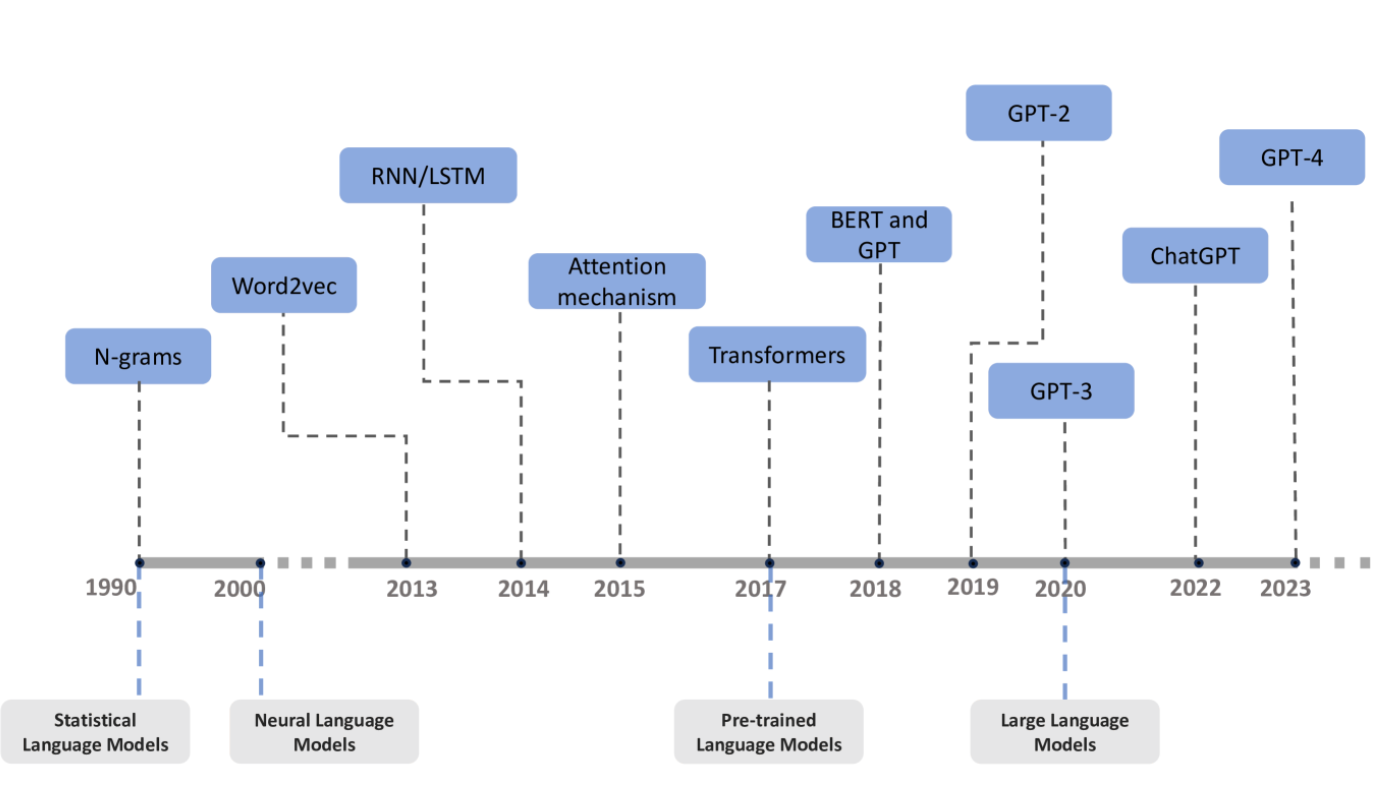
\includegraphics[width=0.8\linewidth]{img/chap04/historyllm.png}
    \caption{History and development of language models}
    \label{fig:historyllm}
\end{figure}

\section{Rule-based Language Model}

In the early days of NLP, rule-based language models were the dominant paradigm for enabling computers to process and generate human language. These models operated on the principle of explicitly programming a set of linguistic rules that dictated how language should be understood or produced. These rules were typically based on grammatical principles, syntactic structures, and semantic relationships that linguists and programmers manually codified.

The core mechanism of a rule-based language model involved defining a system of rules to analyze input text or to generate output text. For natural language understanding (NLU) tasks, these rules might involve pattern matching, keyword identification, and parsing techniques to extract meaning or identify the intent behind a user's input. For natural language generation (NLG) tasks, rules would specify the grammatical structure, word order, and vocabulary to construct coherent and syntactically correct sentences.

Consider a simplified example of a rule-based system for intent classification in a customer service context. Rules could be defined as follows:

\begin{itemize}
    \item If the input contains the keywords "\textit{cancel order}" or "\textit{return item}", classify the intent as "\textit{Order Modification}".
    \item If the input contains the keywords "\textit{track package}" or "\textit{check shipping status}", classify the intent as "\textit{Shipping Inquiry}".
    \item If the input contains the keywords "\textit{change password}" or "\textit{account login}", classify the intent as "\textit{Account Management}".
\end{itemize}

When a user enters a query, the system would scan the input for these predefined keywords and apply the corresponding rule to determine the user's intent.

Similarly, for a basic rule-based system for generating greetings, rules might be:

\begin{itemize}
    \item If the time of day is before 12:00 PM, output "\textit{Good morning}".
    \item If the time of day is between 12:00 PM and 5:00 PM, output "\textit{Good afternoon}".
    \item If the time of day is after 5:00 PM, output "\textit{Good evening}".
\end{itemize}

These examples illustrate the fundamental principle of rule-based models: direct, manual encoding of linguistic knowledge into a set of instructions.

However, these systems suffered from significant limitations. The complexity and variability of natural language made it incredibly difficult to create a comprehensive set of rules that could handle all possible linguistic phenomena. Natural language is full of nuances, exceptions, idiomatic expressions, and context-dependent meanings that are hard to anticipate and program explicitly. As a result, rule-based systems often proved to be brittle and unable to generalize to inputs that deviated even slightly from the predefined patterns. They required extensive manual effort to develop and maintain, and their performance plateaued relatively quickly as the complexity of the language tasks increased.

The foundation of large language models can be traced back to experiments with neural networks and neural information processing systems that were conducted in the 1950s to allow computers to process natural language. Researchers at IBM and Georgetown University worked together to create a system that would be able to automatically translate phrases from Russian to English. As a notable demonstration of machine translation, research in this field took off from there.

The idea of LLMs was first floated with the creation of Eliza in the 1960s: it was the world’s first chatbot, designed by MIT researcher Joseph Weizenbaum. Eliza marked the beginning of research into natural language processing (NLP), providing the foundation for future, more complex LLMs.

ELIZA relies on a pattern-matching algorithm, where the user’s input is parsed for key phrases, and corresponding predefined responses are generated. Its working can be broken down into the following steps:

\begin{itemize}
    \item Input Processing: ELIZA takes user input and searches for specific keywords or phrases.
    \item Pattern Matching: When a match is found, the program applies simple rules to generate a response. These rules are not based on deep understanding but on syntactic structures.
    \item Response Generation: The output is a reformulation of the input, often transformed into a question. If no keywords are detected, ELIZA resorts to generic responses such as “Tell me more” or “Why do you say that?”
\end{itemize}

An example of a conversation with ELIZA could go like this:

User: "I feel sad today."

ELIZA: "Why do you feel sad today?"

This simplistic method created the illusion of understanding and empathy, a hallmark of many early chatbots.

Weizenbaum was attempting to prove his assumption that the communications between humans and machines were fundamentally superficial, but things didn’t work out as planned. To simplify the experiment and minimize disputes, Weizenbaum developed a program using “active listening,” which did not require a database storing real-world information, but would reflect back a person’s statements to carry the conversation forward. 

He was surprised and horrified that people, including Weizenbaum’s own secretary, described the computer program as having human-like feelings. Weizenbaum wrote: “\textit{My secretary, who had watched me work on the program for many months and therefore surely knew it to be merely a computer program, started conversing with it. After only a few interactions with it, she asked me to leave the room}”. He later added, “\textit{I had not realized … that extremely short exposures to a relatively simple computer program could induce powerful delusional thinking in quite normal people}”.

ELIZA’s creation was a pivotal moment in the history of AI, particularly in natural language processing and human-computer interaction. It demonstrated that computers could engage in simulated conversations, paving the way for more complex conversational agents like modern chatbots and voice assistants (e.g., Siri, Alexa, ChatGPT).

Psychological Effects: ELIZA revealed that people were willing to project human-like qualities onto machines, an observation that later became known as the ELIZA effect. Despite the program’s simplistic mechanics, users often felt that ELIZA understood them, highlighting the potential for computers to evoke emotional responses from humans.

Inspiration for Modern Chatbots: ELIZA was the precursor to modern chatbots and virtual assistants that use advanced NLP techniques like deep learning, intent recognition, and context awareness to carry out much more sophisticated interactions.

Ethical Considerations: ELIZA also sparked early discussions about the ethical implications of AI in therapy and other human-centered fields. Weizenbaum himself became critical of using AI in roles that require genuine understanding, like psychotherapy, fearing that people might overestimate the capabilities of such systems.

\section{Statistical Language Models (SLMs)}

The advent of statistical language models (SLMs) in the late 20th century marked a crucial turning point, as these models began to learn language patterns directly from large amounts of data, offering a more flexible and scalable approach that eventually superseded rule-based methods for most NLP applications. Rule-based systems, while historically significant as an initial step in computational language processing, are rarely used as the primary approach today, except in very narrow and well-defined domains where the linguistic scope is highly restricted.

Statistical Language Models, or Count-based models, originated in the 1990s as mathematical models addressing contextually relevant properties of natural language from a probabilistic statistical perspective. 

The essence of statistical language modeling lies in ascertaining the probability of a sentence occurring within a text. Considering $S$ as the sentence "\textit{I am very happy}", $P(w_i)$ signifies the probability of the $i$-th word in the sentence: $w_1$ as "I", $w_2$ as "am", $w_3$ as "very", and $w_4$ as "happy". Now, the objective is to ascertain the likelihood of $S$ appearing in the text, denoted as $P(S)$:

\begin{equation}
P(S) = P(w_1, w_2, w_3, w_4) = P(I, am, very, happy)
\end{equation}

\noindent To calculate this probability, the conditional probability can be employed:

\begin{equation}
P(I, am, very, happy) = P(I) \cdot P(am \mid I) \cdot P(very \mid I, am) \cdot P(happy \mid I, am, very)
\end{equation}

\noindent where $P(I)$ represents the probability of the word ``I" appearing and $P(am \mid I)$ stands for the probability of ``am" appearing given that ``I" has appeared. When we multiply $P(am \mid I)$ by $P(I)$, it fulfills the condition of "I" appearing in $P(am \mid I)$, resulting in the probability of ``I am" appearing together as $P(I, am) = P(I) \cdot P(am \mid I)$. 

\noindent In general, the probability of a sequence of $K$ words is calculated using the chain rule as:

\begin{equation}
P(w_1 w_2 \ldots w_K) = P(w_1) P(w_2 | w_1) \cdots P(w_K | w_1 w_2 \ldots w_{K-1}) = \prod_{k=1}^{K} P(w_k | w_1 w_2 \ldots w_{k-1})
\end{equation}

Now, the question arises: how do we calculate the conditional probability of the occurrence of each word? The answer lies in Maximum Likelihood Estimation, enabling us to estimate probabilities by substituting them with frequencies when the sample size is sufficiently large, given by:

\begin{equation}
P(w_k \mid w_1 w_2 \cdots w_{k-1}) = \frac{P(w_1 \cdots w_{k-1} w_k)}{P(w_1 w_2 \cdots w_{k-1})} = \frac{C(w_1 w_2 \cdots w_k)}{C(w_1 w_2 \cdots w_{k-1})}
\end{equation}

\noindent where $C(\cdot)$ represents the count of occurrences of the subsequence in the training set. Using this formula, we can calculate the likelihood of each word as the $i$-th word given the preceding $k - 1$ words. Then, we select the $k$-th word by choosing the word associated with the highest probability. 

However, the larger $K$ is, the lower the frequency of occurrence of a $K$-word sequence, and there will be cases where the frequency of occurrence of the previous $K - 1$ words is high, causing the probability $P(w_k | w_1 w_2 \ldots w_{k-1})$ to be nearly zero. This leads to the $K$-word sequence almost never occurring (simply put, the sequence does not appear in the training data).\\

\subsection{N-gram Language Model}

To reduce this problem, instead of using $K - 1$ previous words, we only use $N - 1$ previous words (assumes that the $N$-th word is related to the initial $N - 1$ words). This leads us to the concept of \textbf{N-gram Language Models}:

\begin{equation}
    P(w_k | w_1 w_2 \ldots w_{k-1}) = P(w_k | w_{k-N+1} w_{k-N+2} \ldots w_{k-1})
\end{equation}

The probability of a sequence of words is calculated as:

\begin{equation}
    P_N(W) = \prod_{k=1}^{K} P(w_k | w_{k-N+1} w_{k-N+2} \ldots w_{k-1})
\end{equation}

Typically, $N$ is chosen as 1, 2, or 3.\\

This model is also known as a \textbf{(N-1)-order Markov Model}.\\

However, this model has the following drawbacks:

\begin{itemize}
    \item \textbf{Violation of dependency condition}: The transition from $K - 1$ to $N - 1$ is not theoretically valid from the start.
    \item \textbf{Saturation}: With enough data, the model performs better, but at some point, adding more data does not change the probability distribution. This happens especially with bigrams and trigrams, where the number of combinations can reach billions.
    \item \textbf{Lack of generalization}: Different topics, styles, and structures have different word combinations. Thus, with different data sources, model quality varies greatly—especially when training on one type of writing but testing on another. This leads to poor generalization and performance.
\end{itemize}

N-gram model also efficiently computes conditional probabilities. It is necessary to pre-compute and save $C(X)$ required for the conditional probability computation, where $X$ is a sentence of length $n$. The number of possible sentences $X$ grows exponentially with the size of the vocabulary. For instance, with 1000 different words, there exist $1000^n$ potential sequences of length $n$. However, excessively large values of $n$ pose storage limitations. Typically, $n$ is confined to 2 or 3, causing each word to relate to only its first 1 or 2 preceding words, ultimately leading to a reduction in the model’s accuracy.

\subsection{Structured Language Models}

Statistical Language Models have long been central to natural language processing tasks, from speech recognition to machine translation. Traditional SLMs, particularly n-gram models, estimate the probability of a word based on a fixed number of preceding words. Take the previous case as an example, a trigram model might estimate the probability of the word “happy” based on the two previous words of the sentence S: $\mathbf{P}(\text{happy} | \text{am},\text{very})$

While effective for short contexts, n-gram models suffer from significant limitations: they use fixed-length context windows, ignore grammatical structure, and perform poorly when encountering rare or unseen word combinations.

To overcome these challenges, Structured Language Models were introduced. These models extend statistical approaches by incorporating syntactic structures, such as parse trees, into the language modeling process. Rather than treating text as a flat sequence of words, Structured LMs incrementally build syntactic structures as sentences unfold, jointly modeling the likelihood of words and their grammatical relationships.

For example, in the sentence: \textit{The keys to the cabinet are missing}, a traditional trigram model might incorrectly favor “is” over “are” due to its short context. However, a structured LM can parse that “keys” is the true subject of the sentence and correctly predict the plural verb “are” by capturing the syntactic relationship between the subject and verb, regardless of intervening nouns like “cabinet”.

\begin{forest}
  for tree={align=center, parent anchor=south, child anchor=north, l sep=15pt}
  [S
    [$\text{NP}_{pl}$
      [DT [The]]
      [NNS [keys]]
      [PP
        [P [to]]
        [NP
          [DT [the]]
          [NN [cabinet]]
        ]
      ]
    ]
    [$\text{VP}_{pl}$
      [VBP [are]]
      [ADJP
        [VBG [missing]]
      ]
    ]
  ]
\end{forest}

Syntax tree of the sentence "The keys to the cabinet are missing".

Structured LMs offer several key improvements over generic SLMs:

\begin{itemize}
    \item Long-Range Dependency Modeling: Structured LMs are not limited by fixed context windows. They can use hierarchical parse trees to capture dependencies between distant words, improving grammatical coherence.
    \item Better Generalization: By leveraging syntactic roles (e.g., subject, verb, object), Structured LMs generalize better to unseen sequences. Even if a specific phrase hasn’t been encountered during training, its structure may match other known patterns.
    \item Reduced Data Sparsity: Instead of learning from exact word sequences, Structured LMs abstract over syntactic categories. This reduces the zero-probability problem common in high-order n-gram models.
    \item Joint Prediction: Structured LMs jointly predict words, parts-of-speech, and parse decisions, creating a richer and more integrated model of language generation.
\end{itemize}

A well-known example of Structured LM is the model developed by Chelba and Jelinek (2000), which incrementally constructs a binary parse tree while predicting each word in a sentence. This model demonstrated lower perplexity and improved accuracy in speech recognition tasks compared to traditional n-gram baselines.

\section{Neural Language Models (NLMs)}

Neural Language Models leverage neural networks to predict the probabilities of subsequent words within sequences. They effectively handle longer sequences and mitigate the limitations associated with small $n$ in SLMs. 

NLMs operate akin to the n-gram concept, assuming that the probability of each word depends only on its previous $n-1$ words. The first layer—the input layer—concatenates the word vectors of $n-1$ words, forming a vector $X \in \mathbb{R}^{m \times (n-1)}$. Subsequently, the second layer—the hidden layer—derives the output $H$ by applying a non-linear activation function, like sigmoid or tanh, to the matrix product of $X$ and $W_{xh}$. Following this, the third layer—the output layer—aims to forecast the subsequent word based on the hidden layer’s output. With $|V|$ neurons within the output layer, the resulting output vector $O \in \mathbb{R}^{|V|}$ is computed by multiplying $H$ and $W_{ho}$. This resultant vector then undergoes the Softmax function, producing a vector $O'$ containing the probability value assigned to each word.

The Softmax function, concerning the output of the $i$-th neuron, is defined as follows:

\begin{equation}
    O'_i = \text{Softmax}(O'_i) = \frac{\exp(O_i)}{\sum_{j=1}^{|V|} \exp(O_j)}
\end{equation}

\noindent where $O'_i$ denotes the output value of the $i$-th node, and $|V|$ represents the count of output nodes, corresponding to the classification categories. Utilizing the Softmax function allows the transformation of output values from multiclassification into a probability distribution, ensuring a sum of 1 within the range $[0, 1]$.

\begin{figure}[h]
    \centering
    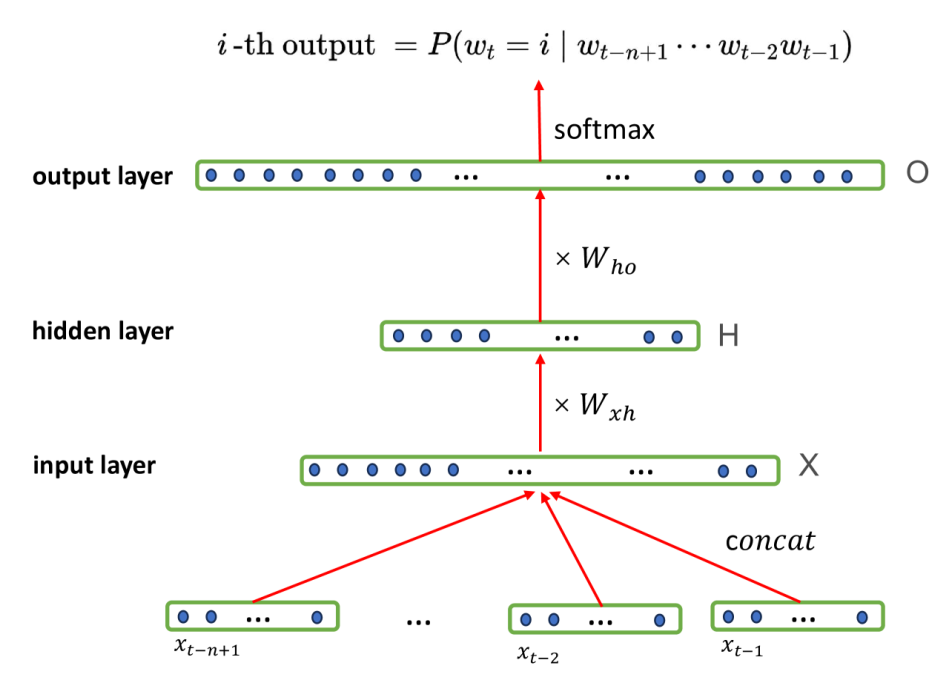
\includegraphics[width=0.8\linewidth]{img/chap04/neuralmodel.png}
    \caption{A Neural Language Model}
    \label{fig:neuralmodel}
\end{figure}

Neural Language Models can solve data sparseness of N-gram Language Models. It can be further classified into Feed Forward Neural Networks (FNNs) and Recurrent Neural Networks (RNNs).

Every NLM has the same kind of input and output:

\begin{itemize}
    \item Input: Word embedding or character embedding (strings and characters to real vectors in an $n-$dimensional space.
    \item Output: For each output unit, it represents the probability of a word or character given the context. What "context" means depends on the type of model being used. For Feedforward Neural Networks (FNNs), the context is a fixed-length sequence consisting of the words or characters immediately preceding the current character being considered. This is similar to N-gram Language Models. For Recurrent Neural Networks (RNNs), the context is like that of FNNs but with variable length. This type helps address the limited context problem of FNNs—meaning it is no longer restricted to N-grams, and the shortcomings of N-gram Language Models are resolved.
\end{itemize}

\textbf{Neural Probabilistic Language Model}

The \textbf{Neural Probabilistic Language Model (NPLM)}, proposed by \textbf{Yoshua Bengio et al. in 2003}, was a landmark in the history of natural language processing (NLP) and deep learning. It was the first major \textit{neural language model}, designed to overcome the limitations of statistical n-gram models, such as:

\begin{itemize}
    \item \textbf{Data sparsity}
    \item \textbf{Poor generalization to unseen sequences}
    \item \textbf{Fixed-size context windows}
\end{itemize}

The NPLM introduced two core innovations:

\begin{enumerate}
    \item \textbf{Word embeddings}: Learn dense vector representations of words.
    \item \textbf{Feedforward neural network}: Predict the next word using the learned embeddings.
\end{enumerate}

\textbf{Model Architecture}

\begin{itemize}
    \item \textbf{Input:} A context of $n-1$ words $(w_1, w_2, \ldots, w_{n-1})$.
    \item \textbf{Embedding Layer:} Each word $w_i$ is mapped to a vector $C(w_i) \in \mathbb{R}^d$. These are concatenated into $x \in \mathbb{R}^{(n-1) \cdot d}$.
    \item \textbf{Hidden Layer:}
    \[
        h = \tanh(Wx + b)
    \]
    where $W$ is the weight matrix, $b$ is a bias vector.
    \item \textbf{Output Layer:}
    \[
        y = b' + Uh
    \]
    where $U$ is the output weight matrix and $b'$ is the bias vector.
    \item \textbf{Softmax Layer:}
    \[
        P(w_t = i \mid w_{t-n+1}, \ldots, w_{t-1}) = \frac{\exp(y_i)}{\sum_{j=1}^{|V|} \exp(y_j)}
    \]
\end{itemize}

\textbf{Key Contributions}

\begin{itemize}
    \item \textbf{Word embeddings}: Represent words in a continuous vector space capturing semantic similarity.
    \item \textbf{Parameter sharing}: Same parameters are used across all word positions, leading to better generalization.
    \item \textbf{Joint learning}: The model learns both word representations and a language model.
\end{itemize}

\textbf{Limitations at the Time}

\begin{itemize}
    \item Computationally expensive due to large vocabulary softmax.
    \item Fixed-size context window; could not model long-range dependencies.
\end{itemize}

These limitations were later addressed by models such as:

\begin{itemize}
    \item \textbf{Word2Vec (2013)}: Efficient embedding training.
    \item \textbf{RNNs, LSTMs}: Sequence modeling with variable context.
    \item \textbf{Transformers}: Parallelized long-range dependency modeling.
\end{itemize}

Reference

Bengio, Y., Ducharme, R., Vincent, P., \& Jauvin, C. (2003). \textit{A Neural Probabilistic Language Model}. Journal of Machine Learning Research, 3(Feb), 1137–1155. \\
\url{https://www.jmlr.org/papers/volume3/bengio03a/bengio03a.pdf}

\textbf{The concept of word vectors}

Humans effortlessly comprehend word meanings. For instance, “cat” and “dog” share closer semantic connections than “cat” and “tree” since they both represent animals. But how does a computer accomplish this? Computers operate using binary code — 0s and 1s — so human language needs translation into binary. Word vectors can accomplish this, which are numerical representations of human language, where each word corresponds to a distinct vector. These vectors usually possess fixed dimensions and can simulate word relationships through the angles between them. An intriguing example is the angle between the word vectors for “cat” and “dog” which is smaller than the angle between the word vector for “cat” and “tree”. Word2Vec is a widely recognized tool for computing word vectors. Its function involves converting words into dense numerical representations, making words with similar semantics closer together in the vector space.

The efficacy of Word2Vec is notably influenced by its utilization of neural networks, which mirrors the structure and functionality of the human brain, comprising interconnected simple units known as neurons organized into different layers. Figure~2 provides a visualization of a simple NLM structure, composed of input, hidden, and output layers. Within this structure, each word vector $x_t \in \mathbb{R}^m$, the matrix $W_{xh} \in \mathbb{R}^{m(n-1) \times h}$, and the matrix $W_{ho} \in \mathbb{R}^{h \times |V|}$, where $h$ signifies the number of neurons in the hidden layer, and $V$ is the vocabulary containing all words recognized by the model.

Word2Vec focuses solely on learning word embeddings rather than modeling full word distributions. This design decision simplifies the model and allows it to scale efficiently.

\textbf{Model Simplification}

Word2Vec uses a shallow neural network with only input and output layers, eliminating hidden layers entirely. It offers two architectures:
\begin{itemize}
    \item \textbf{CBOW (Continuous Bag-of-Words)}: Predicts a word given its context.
    \item \textbf{Skip-Gram}: Predicts context words given a target word.
\end{itemize}

\textbf{Efficient Training with Approximate Objectives}

Instead of using full softmax, Word2Vec employs:

\begin{itemize}
    \item \textbf{Negative Sampling}: Samples a small number of ``negative'' examples for contrastive learning.
    \item \textbf{Hierarchical Softmax}: Uses a binary tree to reduce softmax complexity from $O(|V|)$ to $O(\log |V|)$.
\end{itemize}

These methods drastically reduce training time and memory usage, making it possible to train on corpora with billions of words.

\textbf{Scalability and Practicality}

Due to its lightweight architecture and efficient training, Word2Vec can be applied to very large datasets and has been successfully used to train embeddings on datasets like Google News, Wikipedia, and Common Crawl.

\subsection{Recurrent Neural Network \& Long-Short Term Memory}

Recurrent Neural Networks stand as a cornerstone in the development of artificial intelligence, particularly in the processing of sequential data. Distinct from traditional neural networks, RNNs have the unique ability to retain information from previous inputs, thanks to their internal memory mechanism. This feature makes them exceptionally suitable for tasks where the context and order of data are pivotal, such as in language processing, time series analysis, and speech recognition.

The core functionality of RNNs lies in their looped architecture, which allows information to persist. In an RNN, each unit passes its output back as an input to itself in the subsequent step, creating a form of internal memory. This looping mechanism enables the network to remember past information and use it to influence future outputs. However, this memory is inherently short-lived, a characteristic that serves both as an advantage and a limitation.

RNNs have been effectively employed in a variety of applications where sequential data plays a critical role. In the realm of language modeling and text generation, they can predict the next word in a sentence based on the preceding words. In the field of speech recognition, RNNs are instrumental in understanding the temporal dynamics of spoken language. Additionally, their ability to process time-series data makes them invaluable in areas like stock market prediction and weather forecasting.

Despite their versatility, RNNs face significant limitations, particularly the issue of vanishing gradients. This problem arises when the network struggles to learn and retain information from long sequences, as the gradient—essential for the network's learning process—tends to either vanish or explode during back-propagation through time and layers. This makes it challenging for RNNs to learn long-range dependencies within data sequences.

To address these limitations, a new architecture known as Long Short-Term Memory (LSTM) was developed. LSTMs, while being a type of RNN, include a crucial modification: the incorporation of gates (input, forget, and output gates) that regulate the flow of information. These gates efficiently determine which information should be retained or discarded, enabling LSTMs to maintain longer memory. Consequently, LSTMs can effectively learn from extended sequences of data, significantly enhancing the performance of neural networks in tasks requiring the understanding of long-range dependencies.

Long Short-Term Memory (LSTM) networks have been a significant breakthrough in the field of artificial intelligence, particularly in handling sequences of data. Originating as an advanced form of Recurrent Neural Networks (RNNs), LSTMs were designed to overcome the challenges of learning long-range dependencies, a limitation inherent in traditional RNNs. The key innovation in LSTMs is their use of a gated mechanism, consisting of input, forget, and output gates, which regulates the flow of information. This design allows LSTMs to retain information over longer periods, making them highly effective for complex tasks in natural language processing, speech recognition, and time-series analysis.

While LSTMs represent a significant advancement over traditional RNNs, they are not without their own limitations. One major issue is their computational complexity and inefficiency, primarily due to the sequential nature of their processing. LSTMs struggle with processing very long sequences, as the time and computational resources required scale linearly with the sequence length. Additionally, LSTMs still face challenges with vanishing gradients, albeit to a lesser extent than RNNs, especially in very deep networks or extremely long sequences. This makes them less practical for some real-world applications that involve massive datasets or require rapid processing.

\subsection{Transformers \& Pre-trained Language Models (PLMs)}

The landscape of Natural Language Processing (NLP) underwent a monumental shift with the introduction of the Transformer architecture. This innovative neural network design, detailed in the seminal paper "Attention is All You Need", creatively synthesized ideas from predecessor architectures to overcome their inherent limitations, particularly in handling long-range dependencies in text. The advent of Transformers was not merely an incremental improvement; it laid the foundation for the development of Pre-trained Language Models (PLMs), which have revolutionized how machines understand and generate human language.

Prior to Transformers, Recurrent Neural Networks (RNNs), especially their advanced form, Long Short-Term Memory (LSTM) networks, were the dominant architectures for processing sequential data like text. As we discussed previously, LSTMs addressed the vanishing gradient problem of traditional RNNs through a gated mechanism, enabling them to learn long-range dependencies to some extent. However, LSTMs processed sequences sequentially, which limited their parallelization capabilities and made them computationally expensive for very long sequences.

The Transformer architecture introduced a paradigm shift by primarily relying on the self-attention mechanism. Unlike the sequential processing of RNNs, self-attention allows the model to simultaneously weigh the importance of different words in a sequence when processing a particular word. This mechanism enables the model to directly capture both short and long-range relationships between words, regardless of their distance in the input sequence. The sources highlight that the Transformer model consists of multiple layers of self-attention and feedforward neural networks, which work in concert to learn contextual representations of words and their intricate relationships within a text. This architecture demonstrated superior performance in various NLP tasks and quickly became the backbone of state-of-the-art language models.

\textbf{Understanding Transformer Models: Self-Attention Mechanism}

At the heart of the Transformer model is the self-attention mechanism. This allows the model to process different parts of the input sequence in parallel, as opposed to the sequential processing in RNNs and LSTMs. Self-attention enables the model to weigh the importance of different words in a sentence, regardless of their positional distance from each other. For example, in the sentence "The cat, which was hungry, meowed loudly," the model can directly relate "cat" to "meowed" for better context understanding, something that is more challenging in traditional sequential models.

Architecture Details:

\begin{itemize}
    \item Encoder and Decoder Stacks: The Transformer model consists of an encoder to process the input and a decoder to produce the output. Both the encoder and the decoder are composed of a stack of identical layers, typically six in number.
    \item Encoder: Each encoder layer has two sub-layers. The first is the multi-head self-attention mechanism, and the second is a simple, position-wise fully connected feed-forward network.
    \item Decoder: Each layer in the decoder also has two sub-layers (like the encoder) but adds a third one, which performs multi-head attention over the output of the encoder stack.
    \item Positional Encoding: Since Transformers do not use recurrence, they incorporate positional encodings to give the model information about the relative or absolute position of the words in the sequence. This encoding is added to the input embeddings at the bottoms of the encoder and decoder stacks.
\end{itemize}

\begin{figure}[h]
    \centering
    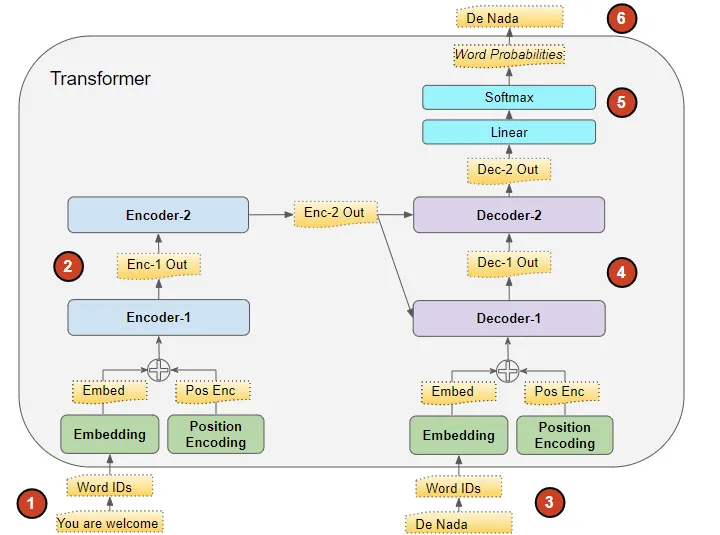
\includegraphics[width=0.8\linewidth]{img/chap04/transformer-arch.png}
    \caption{Architecture of a Transformer}
    \label{fig:transformer-arch}
\end{figure}

Advantages of Transformers:

\begin{itemize}
    \item Parallelization: Unlike RNNs and LSTMs, Transformers process data in parallel, significantly speeding up training.
    \item Handling Long-range Dependencies: Thanks to the self-attention mechanism, Transformers can manage long-range dependencies in text better than RNNs and LSTMs.
    \item Flexibility and Scalability: The architecture is highly flexible and scalable, making it effective for a wide range of tasks beyond NLP, such as image recognition and generation.
\end{itemize}

In this picture is the development by year and the classification of Transformer models:

\begin{figure}[h]
    \centering
    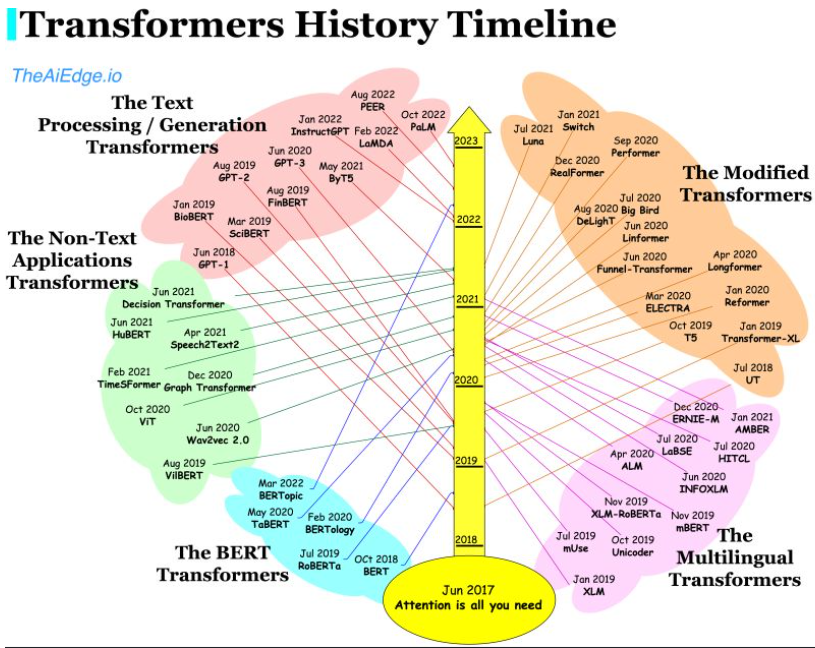
\includegraphics[width=0.8\linewidth]{img/chap04/transformer-history.png}
    \caption{History of Transformers}
    \label{fig:transhist}
\end{figure}

Transformer models have diversified into several distinct classes, each tailored to specific applications and challenges in the field of artificial intelligence.

Processing/Generation Transformers are designed for either interpreting existing text or generating new content. Processing models excel in tasks like sentiment analysis and text classification, adeptly analyzing and extracting insights from language. On the other hand, Generation models are employed for creative tasks like storytelling or text generation, where they generate coherent and contextually relevant text.

In the realm of \textit{Modified Transformers}, various adaptations of the original Transformer architecture aim to enhance performance or efficiency. These models include architectures like the Reformer, which reduces memory consumption, or those with altered attention mechanisms for specific data types or tasks, addressing challenges like handling longer sequences or improving computational efficiency.

\textit{Non-Text Transformers} represent a significant expansion of the Transformer's application, extending beyond traditional natural language processing. These models process data like audio, genomic sequences, or images, leveraging the Transformer architecture to capture complex relationships in non-textual domains. For instance, the Vision Transformer (ViT) adapts the Transformer approach to image processing tasks.

\textit{BERT Transformers}, inspired by Google's BERT, focus on understanding and analyzing language. This class includes models like RoBERTa, DistilBERT, and ALBERT, each building upon or refining the approach of BERT. These models are particularly effective in tasks like text classification, question answering, and language inference, offering deep contextual insights into language.

\textit{Multimodal Transformers} represent a groundbreaking class that processes and generates multiple types of data, such as text and images. Models like OpenAI’s DALL-E and CLIP are prime examples, capable of generating images from text descriptions or understanding concepts across both visual and textual modalities. These models are pioneering in AI, enabling applications like image captioning, visual question answering, and cross-modal translation.

The effectiveness of the Transformer architecture paved the way for the rise of Pre-trained Language Models (PLMs). The principle behind PLMs is to first train a large-scale model on an extensive volume of unlabeled text data to grasp fundamental language structures, including vocabulary, syntax, semantics, and logic – a phase known as pre-training. This pre-training process allows the model to learn general linguistic knowledge from vast amounts of text.

Several training techniques are employed during pre-training. One prominent technique is Masked Language Modeling (MLM), where a certain proportion of tokens in the input sequence are masked, and the model is trained to predict the masked tokens based on the surrounding context. The source indicates that MLM encourages the model to learn meaningful representations of language that can generalize to a wide range of downstream tasks. Another fundamental pre-training objective is Language Modeling (or next token prediction), where the model learns to predict the next word in a sequence given the preceding words.

Once the pre-trained model has acquired a broad understanding of language, it can be adapted to perform specific NLP tasks like text classification, question answering, and text summarization through a process called fine-tuning. Fine-tuning involves further training the pre-trained model on a smaller, task-specific dataset. This "pre-training and fine-tuning" paradigm has proven highly effective, as the pre-trained model's general language knowledge provides a strong foundation for learning task-specific patterns, often requiring significantly less task-specific data and computational resources compared to training models from scratch.

Numerous influential PLMs have emerged based on the Transformer architecture. Models like BERT, which primarily utilizes the MLM objective, excel at tasks requiring a deep understanding of context. The GPT series (including GPT-2, GPT-3, and GPT-4), which employs the next token prediction objective, has demonstrated remarkable capabilities in text generation. Other notable PLMs mentioned in the sources include RoBERTa, PaLM, and LLaMA. These models, trained on massive datasets containing billions of words, have pushed the boundaries of what NLP models can achieve.

The sources highlight several benefits of using PLMs. Their ability to capture general linguistic knowledge allows them to achieve strong performance on a wide range of downstream tasks. The transfer learning capability significantly reduces the need for large amounts of labeled data for each specific task, making NLP more accessible and efficient. Furthermore, the pre-trained weights provide a strong initialization, leading to faster convergence and improved performance during fine-tuning.

To further enhance the efficiency of adapting PLMs, parameter-efficient fine-tuning (PEFT) techniques have been developed. These methods aim to adapt LLMs to specific datasets or domains by updating only a small subset of the model's parameters. Techniques like Adapters, which insert additional learnable layers into the Transformer architecture, and BitFit, which only updates the model's bias terms, allow for efficient fine-tuning while keeping the majority of the pre-trained weights frozen. This approach reduces the computational overhead and memory requirements associated with fine-tuning large models.

The evolution of language models continued with the emergence of Transformer architectures, which have largely surpassed RNNs and LSTMs due to their superior performance on large-scale datasets and their ability to handle long-range dependencies more effectively through the self-attention mechanism. Transformers can selectively attend to key pieces of information in text, allowing for parallel processing and overcoming the sequential processing limitations of RNNs.

Pre-trained Language Models undergo initial training using an extensive volume of unlabeled text, enabling them to grasp fundamental language structures such as vocabulary, syntax, semantics, and logic — a phase termed pre-training. Subsequently, this comprehensive language model can be applied to various NLP tasks like machine translation, text summarization, and questionanswering systems. To optimize its performance, models need to be trained a second time on a smaller dataset customized for a specific downstream task — a phase known as fine-tuning. martial arts principles. A large number of studies on PLMs have been built on this paradigm, which introduces different architectures e.g. GPT-2 and BERT.

\subsection{Large Language Models (LLMs)}

\begin{figure}[h]
    \centering
    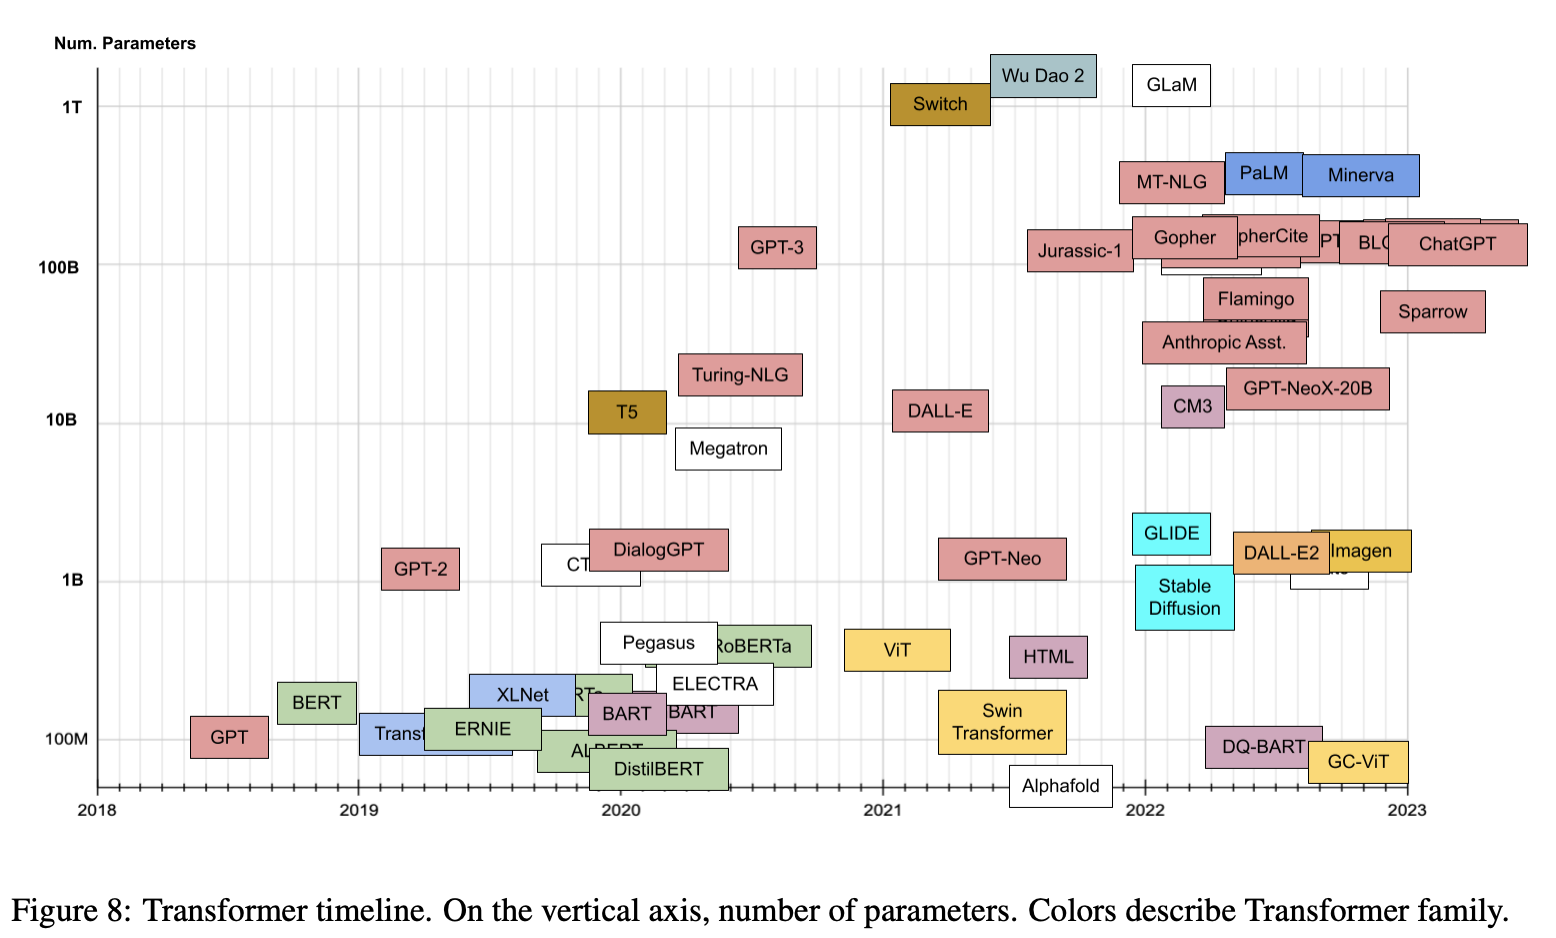
\includegraphics[width=0.8\linewidth]{img/chap04/numparam-transformer.png}
    \caption{Number of parameters of popular Neural Language Models}
    \label{fig:numparam-trans}
\end{figure}

LLMs are trained on massive text corpora with tens of billions (or more) of parameters, such as GPT-3 (Brown et al., 2020), GPT-4 (OpenAI, 2023), PaLM (Chowdhery et al., 2022), and LLaMA (Touvron et al., 2023). The goal of LLMs is to enable machines to understand human commands and adherence to human values. Their hallmark lies in the consolidation of two stages: initial pre-training on a vast general-purpose corpus followed by alignment with human values, rather than transitioning to a different domain. LLMs exhibit remarkable adaptability compared to PLMs, transitioning from specialized to general-purpose models. The substantial increase in model size, dataset volume, and computational prowess has resulted insignificant enhancements across various tasks and unveiled remarkable capabilities absent in smaller models. For example, GPT-3 has the capability to leverage contextual information, a functionality that GPT-2 (Radford et al., 2019) lacks. This means that when GPT-3 is prompted with task-related examples, it utilizes them to enhance its problem-solving capabilities. The number of parameters for LLMs typically exceeds a hundred billion, and the training data is usually in the range of a few hundred GB to a few TB. A concrete example is that there are multiple versions of the GPT-2 model, with the largest version having 1.5 billion parameters and using 40GB of text data for training. In contrast, the largest version of the GPT-3 model has 175 billion parameters and uses 570GB of text data for training. This example illustrates the significant discrepancy between LLMs and PLMs concerning parameter count and training data volume.

The field of Natural Language Processing (NLP) has witnessed a remarkable evolution, culminating in the emergence of Large Language Models (LLMs). These sophisticated AI systems represent a significant leap forward in the ability of machines to understand, generate, and interact with human language. Building upon decades of research in language modeling, LLMs have captured widespread attention due to their impressive capabilities across a diverse range of tasks. To comprehend their impact, it is crucial to define what constitutes an LLM and to identify prominent examples based on the available sources.

Large Language Models (LLMs) can be understood as an extension of PLMs, characterized primarily by their massive scale in terms of number of parameters (often tens of billions or more) and the extensive datasets they are trained on. This increase in scale, coupled with advancements in computational power and algorithmic innovations, has led to emergent abilities and significantly enhanced performance compared to their predecessors. The goal of LLMs is to understand human commands and align with human values. They often exhibit remarkable adaptability, transitioning from specialized to general-purpose models.

The architecture that underpins many state-of-the-art LLMs is the Transformer. As discussed in the previous section, the Transformer architecture, with its reliance on the self-attention mechanism, allows the model to efficiently capture both short and long-range dependencies in text, overcoming the limitations of earlier sequential models like RNNs and LSTMs. The ability to process information in parallel and to weigh the importance of different words in a sequence has been crucial in enabling LLMs to handle vast amounts of data and learn complex linguistic structures.

The sources provide numerous examples of LLMs that exemplify these characteristics:

\begin{itemize}
    \item The GPT series of models (GPT-3, GPT-4) from OpenAI are frequently cited as prominent examples of LLMs. These models, trained on massive textual data, have demonstrated the ability to generate human-level text and perform language-based tasks with exceptional precision. GPT-4, in particular, has shown strong performance in professional exams and explaining legal concepts.
    \item PaLM (Pathways Language Model) is another LLM highlighted in the sources. It has been noted for its performance and is used in the Bard chatbot service.
    \item LLaMA (Large Language Model Meta AI) is mentioned as an open-source LLM trained on publicly accessible datasets. Smaller versions of LLaMA have been fine-tuned for specific tasks like medical question answering (ChatDoctor). Recently, LLaMA 2 has also been released.
    \item BloombergGPT is presented as a specialized LLM with 50 billion parameters, designed to excel in financial tasks while maintaining strong general language model performance.
    \item Other LLMs mentioned include LaMDA, a family of chatbot LLMs from Google, and open-access multilingual models like BLOOM.
\end{itemize}

The capabilities of LLMs are wide-ranging, spanning areas such as customer support through automated responses, content creation for articles and creative writing, computer programming through code generation, and research assistance by rapidly retrieving and summarizing information. They are being applied in specialized domains like medicine for medical question answering and information extraction, and law for legal question answering and text generation.

Despite their impressive advancements, the sources also highlight several limitations of LLMs. These include the issue of hallucinations, where LLMs generate incorrect or non-existent information, prompt brittleness, where slight changes in the input prompt can significantly affect the output, the potential for biases due to the data they are trained on, and the challenges in detecting generated text which can have implications for misinformation and plagiarism.

In conclusion, Large Language Models (LLMs) are a class of language models characterized by their vast number of parameters and training on massive datasets, often utilizing the Transformer architecture. This scale enables them to exhibit emergent abilities and achieve state-of-the-art performance across a wide range of NLP tasks. Examples such as the GPT series, PaLM, LLaMA, and BloombergGPT demonstrate the diverse applications and ongoing advancements in this rapidly evolving field. While holding immense potential, it is crucial to acknowledge and address the inherent limitations of LLMs to ensure their responsible development and deployment.

\textbf{Milestones in LLM Development: GPT, BERT, XLNet, T5, and Beyond
}

Several milestones have marked the evolution of LLM systems, each contributing to
advancements in language understanding, generation, and representation learning:

\begin{enumerate}
    \item GPT (Generative Pre-trained Transformer)

Introduced by OpenAI in 2018, the GPT series represented a significant leap forward in LLM development. GPT-1 demonstrated the efficacy of largescale pre-training on diverse text corpora followed by fine-tuning on specific downstream tasks. Subsequent iterations, such as GPT-2 and GPT-3, increased model size and performance, with GPT-3 achieving remarkable capabilities in natural language generation and understanding.

\begin{figure}[h]
    \centering
    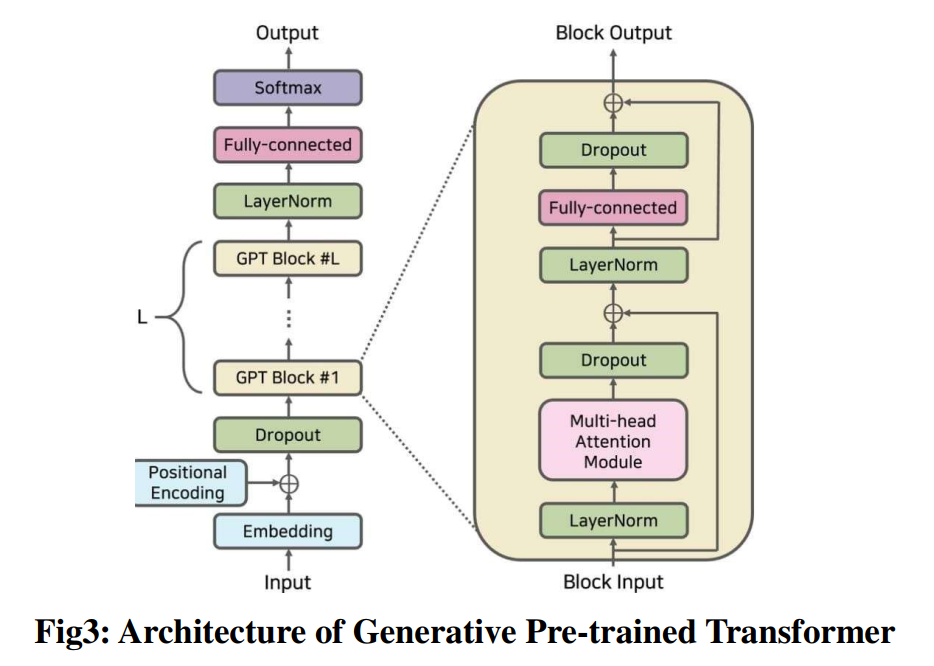
\includegraphics[width=0.8\linewidth]{img/chap04/gptstructure.png}
    \caption{Architecture of Generative Pre-trained Transformer}
    \label{fig:gptarch}
\end{figure}

    \item BERT (Bidirectional Encoder Representations from Transformers)

Released by Google in 2018, BERT revolutionized NLP by introducing a bidirectional pre-training approach. Unlike previous models that processed text sequentially, BERT leveraged masked language modelling and next sentence prediction tasks to capture contextual information bidirectionally. This enabled BERT to achieve stateof-the-art performance on a wide range of NLP tasks, including sentiment analysis, named entity recognition, and question answering.

\begin{figure}[h]
    \centering
    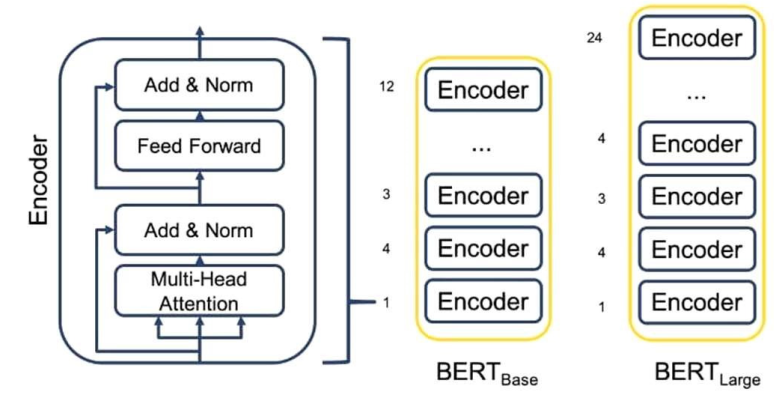
\includegraphics[width=0.8\linewidth]{img/chap04/bertarch.png}
    \caption{Bidirectional Encoder Representation from Transformer's Architecture}
    \label{bertarch}
\end{figure}

\item XLNet

Introduced by researchers at Google AI in 2019, XLNet further advanced the stateof-the-art in LLMs by addressing limitations of previous models such as token-level permutation and context fragmentation. XLNet employed a permutation-based training objective, allowing it to capture bidirectional context while maintaining the advantages of autoregressive  language modelling. This approach resulted in improved performance on various benchmark tasks, surpassing previous models like BERT.

\begin{figure}[h]
    \centering
    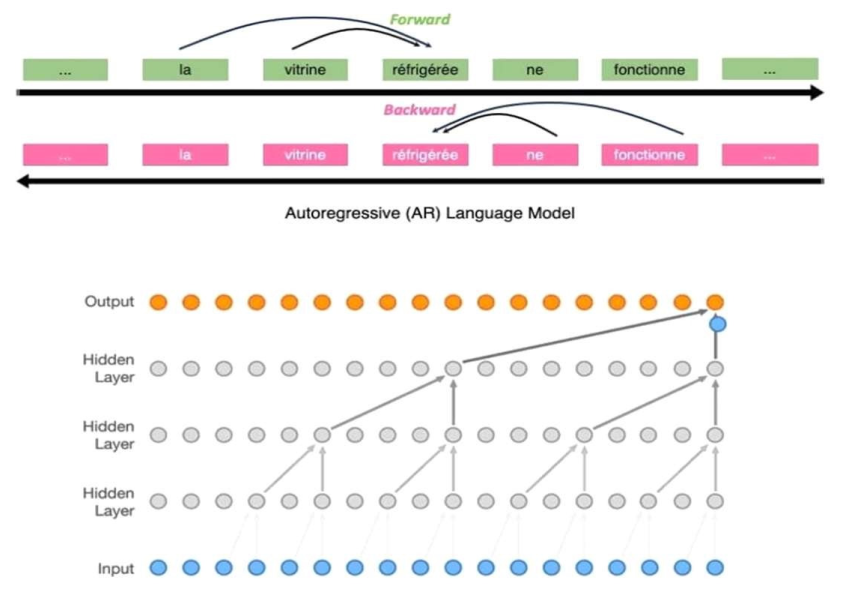
\includegraphics[width=0.8\linewidth]{img/chap04/xlnet-arch.png}
    \caption{Understanding language using XLNET with autoregressive pre-training}
    \label{fig:xlnet-arch}
\end{figure}

\item T5 (Text-To-Text Transfer Transformer)

Developed by researchers at Google AI in 2019, T5 introduced a unified framework for NLP tasks by formulating them as text-to-text transformations. Unlike traditional models that were designed for specific tasks, T5 could perform multiple tasks, including translation, summarization, question answering, and text classification, by simply altering the input-output format. This approach simplified model architecture and training, leading to more efficient and versatile LLMs.
\begin{figure}[h]
    \centering
    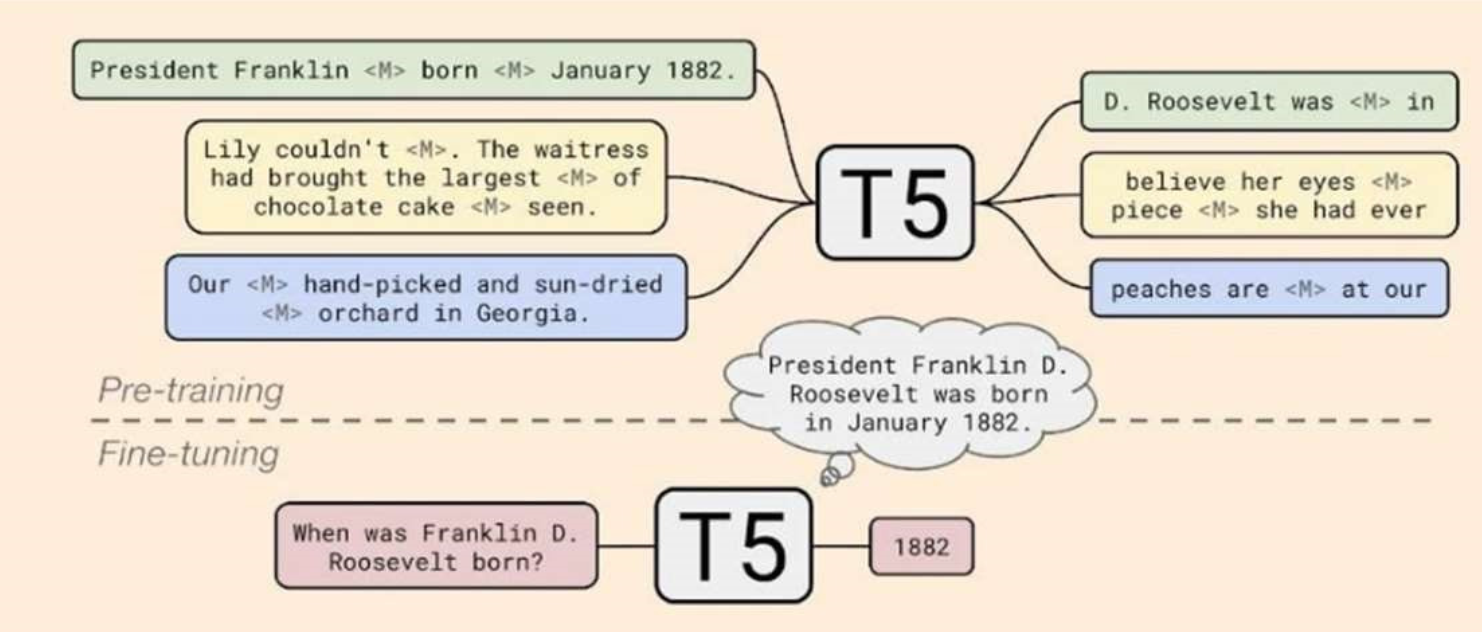
\includegraphics[width=0.8\linewidth]{img/chap04/t5arch.png}
    \caption{Google Text-to-Text Transfer Transformer(T5)}
    \label{fig:t5-arch}
\end{figure}

\end{enumerate}


\subsection{LLM Agents}

One of the bigger frontiers in LLM research is the creation of agents. ChatGPT and similar platforms can generate API calls and functioning code, but humans still need to copy and paste the code to actually do anything with it.

Agents are meant to get around this limitation. Auto-GPT, for example, pairs an underlying LLM with a “bot” that takes high-level tasks, breaks them down into tasks an LLM can solve, and stitches together those solutions. The integration of LLMs into AI agents has significantly advanced their performance, enabling more complex reasoning and decision-making processes. These agents can now autonomously navigate tasks such as web browsing, information synthesis, and report generation, effectively augmenting white-collar work. For instance, OpenAI's Deep Research agent exemplifies this progression by autonomously exploring the web, selecting pertinent information, and compiling detailed reports.

\subsection{Multimodal Models}

Another development worth mentioning is the rise of multi-modality. A model is “multi-modal” when it can process more than one kind of information, like images and text.

LLMs are staggeringly good at producing coherent language, and image models could do the same thing with images, but now a lot of time and effort is being spent on combining these two kinds of functionality.

The result has been models able to find specific sections of lengthy videos, generate images to accompany textual explanations, and create their own incredible videos from short, simple prompts.

Multimodal models extend the capabilities of traditional LLMs by integrating and processing multiple data modalities, such as text, images, audio, and video. This integration enables a more comprehensive understanding and generation of content across various formats. The progression towards Multimodal Large Language Models (MLLMs) represents a significant advancement in AI, facilitating applications that require simultaneous interpretation of diverse data types. For example, Meta's Llama 3.2 model can process visual information, enabling applications in robotics and virtual reality. 
The incorporation of multimodal capabilities into LLMs has led to models that can perform tasks such as visual grounding, image generation and editing, and comprehensive content understanding. This evolution reflects a broader trend towards creating AI systems capable of more nuanced and context-rich interactions. 

% \section{Factors Propelling the Evolution of LLMs}


% \section{\textbf{Increased Data Diversity and Volume}}


% \section{\textbf{Computational Advancements}}


% \section{\textbf{Algorithmic Innovations: The Transformer Architecture}}

% \section{Key Architectural and Training Innovations}


% \section{\textbf{The Transformer Model and Self-Attention}}


% \section{Pre-training Objectives (e.g., MLM, Prefix LM)}


% \section{Scaling Laws and Compute-Optimal Training}


% \section{Advancements in Context Length}


% \section{Techniques for Efficient Training and Inference}


% \section{Impact and Applications Across Domains}


% \section{Natural Language Processing Tasks}


% \section{Creative Work and Knowledge Work}


% \section{Science, Medicine, and Law}


% \section{Robotics and Embodied Agents}


% \section{Synthetic Data Generation}


% \section{Ongoing Challenges and Future Directions}


% \section{Behavioral Challenges (e.g., Hallucinations, Misalignment)}


% \section{Scientific Challenges (e.g., Reproducibility)}


% \section{Ethical Considerations}


% \section{Towards More Capable and Reliable LLMs}

\newpage 
